\section{Testovanie a vyhodnotenie}
\label{sec:test}

% ----- Funkčné testovanie klienta -----
\subsection{Funkčné testovanie klienta}

Klientska aplikácia sa overila automatizovaným testom v prehliadači Microsoft
Edge (skript s knižnicou Playwright, ktorý ovládal skutočnú aplikáciu
spustenú vývojovým serverom). Volania API sa v tomto teste nahradili
pripravenými odpoveďami, takže test overuje klienta, nie server.
Výsledky sú v Tab.~\ref{tab:func}.

% Tabuľka: Výsledky funkčného testu klienta.
\begin{table}[!htbp]
  \centering
  \small
  \caption{Výsledky funkčného testu klienta.}
  \label{tab:func}
  \begin{tabularx}{\textwidth}{|Y|M{2.4cm}|}
    \hline
    \rowcolor[gray]{0.9} \textbf{Kontrolovaná vlastnosť} & \textbf{Výsledok} \\
    \hline
    Tlačidlo „Začať meranie“ je neaktívne bez mena a súhlasu & splnené \\
    \hline
    Vstupné pole je po prechode na meranie aktívne (fokus) & splnené \\
    \hline
    Nesprávny text sa zamietne, pole sa vyprázdni a zobrazí sa chyba & splnené \\
    \hline
    Správny pokus sa započíta a zvýši počítadlo & splnené \\
    \hline
    Po 15 pokusoch sa zobrazí súhrn (15 pokusov) & splnené \\
    \hline
    Odoslaná relácia obsahuje $15 \times 74 = 1110$ udalostí & splnené \\
    \hline
    Odoslanie vráti potvrdenie, tlačidlo „Späť“ zachová zadané meno & splnené \\
    \hline
    Režim identifikácie zobrazí výsledok a umožní ho zopakovať & splnené \\
    \hline
    Chyby v konzole prehliadača & žiadne \\
    \hline
  \end{tabularx}
\end{table}

Počet udalostí vyplýva z toho, že jeden pokus s vetou má 37 stlačení a 37
uvoľnení, teda 74 udalostí (pri slove je to 20).

Tento test sa vykonal pred zavedením režimu slova. Neskoršie zmeny
(automatické uloženie relácie, okamžité zrušenie pokusu pri Backspace alebo
nesprávnom znaku, výber režimu) sa overili
prekladom klienta, ručným vyskúšaním režimu slova a simuláciou komponentu
merania v prostredí jsdom (nesprávny znak vyprázdni pole a zobrazí
hlásenie); automatizovaný test v prehliadači sa po týchto zmenách
neopakoval.

% ----- Vyhodnotenie identifikácie -----
\subsection{Vyhodnotenie identifikácie}

Metóda identifikácie sa vyhodnocuje podľa protokolu z podkapitoly~\ref{sec:protokol}:
šablóny z pokusov 1--10, testovanie na pokusoch 11--15. Vyhodnotenie
vracia koncový bod \code{/api/evaluation}.

\paragraph{Zozbierané dáta.}
Údaje o súbore dát (stav databázy k 20.~11.~2026) sú v Tab.~\ref{tab:data}. Mená účastníkov sú v tejto
práci nahradené označeniami Účastník 1 až 5 (traja z účastníkov sú autormi práce;
číslovanie je náhodné).

% Tabuľka: Charakteristika zozbieraných dát.
\begin{table}[!htbp]
  \centering
  \small
  \caption{Charakteristika zozbieraných dát.}
  \label{tab:data}
  \begin{tabularx}{\textwidth}{|Y|M{6cm}|}
    \hline
    \rowcolor[gray]{0.9} \textbf{Ukazovateľ} & \textbf{Hodnota} \\
    \hline
    Počet účastníkov & 5 \\
    \hline
    Počet relácií & 14 (9 s vetou, 5 so slovom) \\
    \hline
    Počet zaznamenaných klávesových udalostí & 11\,560 \\
    \hline
    Počet testovacích pokusov (11--15) vo vyhodnotení (veta) & 38 \\
    \hline
    Zloženie podľa zariadenia (notebook / stolný počítač) & notebook: 14 relácií, stolný počítač: 0 \\
    \hline
    Zloženie podľa klávesnice (vstavaná / USB / Bluetooth) & vstavaná: 7 relácií, externá USB: 7 relácií, Bluetooth: 0 \\
    \hline
  \end{tabularx}
\end{table}

Počty relácií a udalostí pochádzajú z koncového bodu \code{/api/stats} a zahŕňajú aj päť relácií s režimom slova (tri od
Účastníka~1 na externej USB klávesnici a po jednej od Účastníka~3
a Účastníka~5 so vstavanou klávesnicou). Vyhodnotenie
identifikácie v tejto podkapitole sa týka režimu vety, teda deviatich relácií.
Všetky relácie sa zaznamenali na notebooku. Vo vete sú štyri relácie
s externou USB klávesnicou (tri relácie Účastníka~5 a jedna relácia Účastníka~2)
a päť so vstavanou klávesnicou; vplyv zariadenia sa preto nedá vyhodnotiť
a vplyv klávesnice len veľmi obmedzene.
V režime vety majú štyria účastníci po jednej relácii, Účastník~5 má relácií päť.
Z nich je jedna celá neplatná (38 až 39 stlačení namiesto 37 v každom pokuse)
a v ďalšej je neplatný jeden pokus (tretí, v časti určenej na šablónu). Pri
Účastníkovi~1 sú dva testovacie pokusy neplatné (39 stlačení namiesto 37,
čo zodpovedá jednému preklepu a jeho oprave klávesom Backspace). Neplatné
pokusy sa pri tvorbe šablón aj vo vyhodnotení ignorujú
(podkapitola~\ref{sec:priznaky}).

\paragraph{Úspešnosť.}
Výsledky z koncového bodu \code{/api/evaluation} sú v Tab.~\ref{tab:vysledky}.

% Tabuľka: Úspešnosť identifikácie na testovacích pokusoch 11--15.
\begin{table}[!htbp]
  \centering
  \small
  \caption{Úspešnosť identifikácie (pokusy 11--15)}
  \label{tab:vysledky}
  \begin{tabularx}{\textwidth}{|Y|M{3.5cm}|}
    \hline
    \rowcolor[gray]{0.9} \textbf{Metrika} & \textbf{Hodnota} \\
    \hline
    Počet testovacích pokusov (\code{total}) & 38 \\
    \hline
    Správne na prvom mieste & 30 \\
    \hline
    Top-1 (\code{top1}) & 78,95\,\% \\
    \hline
    Správny účastník medzi prvými tromi & 37 \\
    \hline
    Top-3 (\code{top3}) & 97,37\,\% \\
    \hline
  \end{tabularx}
\end{table}

Úspešnosť podľa účastníka uvádza Tab.~\ref{tab:participant} a maticu zámen
Tab.~\ref{tab:confusion} (v riadkoch je skutočný účastník, v stĺpcoch predikcia). Pokus
označený ako neznámy sa počíta ako chybný.

% Tabuľka: Úspešnosť top-1 podľa účastníka.
\begin{table}[!htbp]
  \centering
  \small
  \caption{Úspešnosť top-1 podľa účastníka.}
  \label{tab:participant}
  \begin{tabularx}{\textwidth}{|Y|C|C|C|}
    \hline
    \rowcolor[gray]{0.9} \textbf{Účastník} & \textbf{Testovacích pokusov} & \textbf{Správne} & \textbf{Top-1} \\
    \hline
    Účastník 1 & 3 & 2 & 66,7\,\% \\
    \hline
    Účastník 2 & 5 & 4 & 80,0\,\% \\
    \hline
    Účastník 3 & 5 & 5 & 100,0\,\% \\
    \hline
    Účastník 4 & 5 & 2 & 40,0\,\% \\
    \hline
    Účastník 5 & 20 & 17 & 85,0\,\% \\
    \hline
    Spolu & 38 & 30 & 78,9\,\% \\
    \hline
  \end{tabularx}
\end{table}

% Tabuľka: Matica zámen (riadky: skutočný účastník, stĺpce: predikcia).
\begin{table}[!htbp]
  \centering
  \small
  \caption{Matica zámen}
  \label{tab:confusion}
  \begin{tabularx}{\textwidth}{|Y|C|C|C|C|C|C|}
    \hline
    \rowcolor[gray]{0.9}  & \textbf{Úč.~1} & \textbf{Úč.~2} & \textbf{Úč.~3} & \textbf{Úč.~4} & \textbf{Úč.~5} & \textbf{neznámy} \\
    \hline
    Účastník 1 & 2 & 1 & 0 & 0 & 0 & 0 \\
    \hline
    Účastník 2 & 0 & 4 & 0 & 0 & 0 & 1 \\
    \hline
    Účastník 3 & 0 & 0 & 5 & 0 & 0 & 0 \\
    \hline
    Účastník 4 & 0 & 0 & 3 & 2 & 0 & 0 \\
    \hline
    Účastník 5 & 0 & 0 & 3 & 0 & 17 & 0 \\
    \hline
  \end{tabularx}
\end{table}

Platia tu aj obmedzenia z podkapitoly~\ref{sec:obmedzenia}. Vzorka je malá (38 pokusov), takže jeden
pokus mení top-1 približne o 3 percentuálne body. Počet pokusov na účastníka
je nerovnaký: Účastník~5 prispieva 20 z 38 pokusov, takže celkové čísla sú
ním výrazne ovplyvnené. Pri piatich účastníkoch so šablónou by náhodný
odhad dosiahol top-1 20\,\% a top-3 60\,\%.

\paragraph{Postup na získanie čísel.} Po zbere dát spustite server a
otvorte v prehliadači adresu \code{/api/evaluation} servera; odpoveď
obsahuje polia \code{top1}, \code{top3}, \code{total} a \code{confusion}.
Údaje o súbore dát poskytujú \code{/api/stats} a \code{/api/sessions}.

% ----- Príklad identifikácie jedného pokusu -----
\subsection{Príklad identifikácie jedného pokusu}
\label{sec:priklad-real}

Postup z podkapitoly~\ref{sec:priklad} je ďalej ukázaný na jednom skutočnom
testovacom pokuse (15. pokus tretej relácie Účastníka~5, teda pokus mimo
šablóny). Pokus bol vybraný ako ilustračný, nie ako typický: ide o jeden
z pokusov, pri ktorých sa v prvej trojke objavili práve traja účastníci,
ktorí sú autormi práce. Čísla v Tab.~\ref{tab:priklad-real} vrátila funkcia
identifikácie servera. Pokus mal 37 stlačení, vektor $m=73$ príznakov a celkový
čas písania približne 7,2\,s.

% Tabuľka: Skutočný výsledok identifikácie jedného testovacieho pokusu.
\begin{table}[!htbp]
  \centering
  \small
  \caption{Identifikácia jedného testovacieho pokusu}
  \label{tab:priklad-real}
  \begin{tabularx}{\textwidth}{|Y|C|C|C|}
    \hline
    \rowcolor[gray]{0.9} \textbf{Poradie a účastník} & \textbf{Vzdialenosť $d_i$} & \textbf{Váha $w_i=1/d_i$} & \textbf{Miera podobnosti $p_i$} \\
    \hline
    1. Účastník 5 & 4,955 & 0,2018 & 64,6\,\% \\
    \hline
    2. Účastník 3 & 16,535 & 0,0605 & 19,4\,\% \\
    \hline
    3. Účastník 1 & 20,016 & 0,0500 & 16,0\,\% \\
    \hline
  \end{tabularx}
\end{table}

Skutočný autor pokusu je na prvom mieste. Kontrola neznámeho pokusu podľa
vzorca~\eqref{eq:unknown} dáva $d_{\min}/\sqrt{m} = 4{,}955/\sqrt{73} \approx 0{,}58$,
čo je výrazne menej ako prah 3, takže pokus sa neoznačí ako neznámy. Rozdiel
vzdialeností medzi prvým a druhým účastníkom je výrazný (5,0 oproti 16,5);
64,6\,\% je len relatívny podiel medzi tromi najbližšími šablónami
(vzorec~\eqref{eq:share}).

% ----- Diskusia -----
\subsection{Diskusia}

Z Tab.~\ref{tab:confusion} vyplývajú tieto pozorovania. Osem z 38 pokusov
bolo určených nesprávne: tri pokusy Účastníka~4 a tri pokusy Účastníka~5 boli
priradené Účastníkovi~3, jeden pokus Účastníka~1 bol priradený Účastníkovi~2
a jeden pokus Účastníka~2 bol označený ako neznámy. Šesť z ôsmich chýb
teda smeruje k Účastníkovi~3, ktorý bol sám rozpoznaný vo všetkých piatich
pokusoch. V jednom prípade z 38 nebol správny účastník ani medzi prvými
tromi (top-3 je 37 z 38).

Účastník~5 dosiahol 85,0\,\% (17 z 20) na pokusoch zo štyroch platných relácií.
Najslabšie je rozpoznaný Účastník~4 (40\,\%), ktorého
pokusy sa najčastejšie zamieňajú s Účastníkom~3.

% ----- Príčiny zámen -----
\paragraph{Príčina zámen.}
Zámeny smerujúce k Účastníkovi~3 sa dajú vysvetliť šírkou jeho šablóny.
Štandardizovaná vzdialenosť (vzorec~\eqref{eq:dist}) delí odchýlku od
priemeru smerodajnou odchýlkou šablóny, takže široká šablóna zmenšuje
vzdialenosť aj pre pokusy iných účastníkov a priťahuje ich k sebe. Údaje
v Tab.~\ref{tab:sigma} to podporujú: šablóna Účastníka~3 má najväčšiu
priemernú smerodajnú odchýlku príznakov (145,7\,ms, u Účastníkov~1 a~5 len
51,0 a 53,5\,ms) a cudzie pokusy sú k nej v priemere najbližšie
($d/\sqrt{m} = 2{,}32$ oproti 3,39 až 6,76 pri ostatných šablónach).
Účastník~3 píše aj najpomalšie (pokus mu trvá približne 21\,s, ostatným 8 až 15\,s).
Účastník~2 má tiež širokú šablónu (140,4\,ms), no priťahuje len jednu zámenu,
takže šírka šablóny nie je jediný činiteľ.

% Tabuľka: Šírka šablón a vzdialenosť cudzích pokusov.
\begin{table}[!htbp]
  \centering
  \small
  \caption{Šírka šablón a vzdialenosť cudzích pokusov}
  \label{tab:sigma}
  \begin{tabularx}{\textwidth}{|Y|C|C|C|}
    \hline
    \rowcolor[gray]{0.9} \textbf{Účastník} & \textbf{Priem. smerodajná odchýlka šablóny [ms]} & \textbf{Priem. čas pokusu [s]} & \textbf{Priem. $d/\sqrt{m}$ cudzích pokusov} \\
    \hline
    Účastník 1 & 51,0 & 8,7 & 4,35 \\
    \hline
    Účastník 2 & 140,4 & 15,1 & 3,39 \\
    \hline
    Účastník 3 & 145,7 & 21,2 & 2,32 \\
    \hline
    Účastník 4 & 63,6 & 12,8 & 6,76 \\
    \hline
    Účastník 5 & 53,5 & 7,9 & 6,67 \\
    \hline
  \end{tabularx}
\end{table}

Domnienku sme overili aj jednoduchým pokusom: namiesto smerodajnej odchýlky
každej šablóny sme pre všetkých účastníkov použili spoločnú odchýlku (priemer
odchýlok všetkých šablón, teda bez údajov z testovacích pokusov). Top-1 vtedy
vzrástol z 31 na 37 z 38 pokusov (97,4\,\%) a top-3 na 38 z 38; zostala jediná
chyba (pokus Účastníka~5 priradený Účastníkovi~4) a žiadna už nesmeruje
k Účastníkovi~3. Porovnanie je bez pravidla pre neznámy pokus, preto je
základ 31 z 38 a nie 30 z 38. Ide o jeden pokus na malej vzorke, nie o hotové
vylepšenie metódy; do implementácie sa nezaviedol.

% ----- Obmedzenia vyhodnotenia -----
Vplyv zariadenia sa nedá posúdiť, pretože všetky relácie vznikli na
notebooku; vplyv klávesnice sa nedá oddeliť od vplyvu osoby (tri zo štyroch
relácií vety s externou USB klávesnicou patria jednému účastníkovi). Šablóna sa
počíta z desiatich pokusov s 73 príznakmi, takže odhad smerodajnej odchýlky
je nepresný. Pri troch až piatich testovacích pokusoch na osobu (Účastník~5 ich
má 20) mení jeden pokus úspešnosť účastníka o 20 až 33 percentuálnych bodov,
preto rozdiely medzi účastníkmi (od 40\,\% do 100\,\%) treba vnímať opatrne.
Účastník~1 má navyše len tri testovacie pokusy, pretože dva boli neplatné pre
opravu klávesom Backspace. Jediný pokus označený ako neznámy patrí účastníkovi,
ktorý bol inak správne rozpoznaný; prah~3 pri identifikácii by sa preto mal kalibrovať
podobne ako prah v analýze overenia (podkapitola~\ref{sec:kalibracia}).

% ----- Chyby overenia a kalibrácia prahu -----
\subsection{Chyby overenia a kalibrácia prahu}
\label{sec:kalibracia}

Analýza z podkapitoly~\ref{sec:overenie} sa vykonala skriptom
\code{backend/far\_frr.py} na rovnakých dátach ako identifikácia v režime vety
(5 účastníkov, 38 testovacích pokusov, stav databázy k 20.~11.~2026).
Tab.~\ref{tab:kalibracia} uvádza počty porovnaní a vybraný prah,
Tab.~\ref{tab:chyby-overenia} chyby na pokusoch 14--15, ktoré sa pri výbere prahu
nepoužili. Obr.~\ref{fig:farfrr} ukazuje krivky FAR a FRR podľa prahu
a Obr.~\ref{fig:skore} rozdelenie skóre vlastných a cudzích porovnaní. Na
Obr.~\ref{fig:farfrr} je zelená čiara kalibrovaný prah a prerušovaná čiara pôvodný
prah 3; na Obr.~\ref{fig:skore} sú hodnoty nad 8 započítané do posledného stĺpca.

% Tabuľka: Kalibrácia prahu overenia (režim vety).
\begin{table}[!htbp]
  \centering
  \small
  \caption{Kalibrácia prahu overenia (režim vety).}
  \label{tab:kalibracia}
  \begin{tabularx}{\textwidth}{|Y|M{3.5cm}|}
    \hline
    \rowcolor[gray]{0.9} \textbf{Ukazovateľ} & \textbf{Hodnota} \\
    \hline
    Kalibračné porovnania (pokusy 11--13), vlastné & 22 \\
    \hline
    Kalibračné porovnania (pokusy 11--13), cudzie & 88 \\
    \hline
    Kalibrovaný prah $\tau^{*}$ & 2,13 \\
    \hline
    EER na kalibračných pokusoch & 13,6\,\% \\
    \hline
    Testovacie porovnania (pokusy 14--15), vlastné / cudzie & 16 / 64 \\
    \hline
  \end{tabularx}
\end{table}

% Tabuľka: Chyby overenia na nezávislých pokusoch 14--15 pri pôvodnom a kalibrovanom prahu.
\begin{table}[!htbp]
  \centering
  \small
  \caption{Chyby overenia na pokusoch 14--15}
  \label{tab:chyby-overenia}
  \begin{tabularx}{\textwidth}{|Y|C|C|}
    \hline
    \rowcolor[gray]{0.9} \textbf{Prah} & \textbf{FAR} & \textbf{FRR} \\
    \hline
    pôvodný, $\tau = 3$ & 35,9\,\% & 12,5\,\% \\
    \hline
    kalibrovaný, $\tau^{*} = 2{,}13$ & 10,9\,\% & 18,8\,\% \\
    \hline
  \end{tabularx}
\end{table}

% Obrázok (graf z backend/far_frr.py): krivky FAR a FRR.
\begin{figure}[H]
  \centering
  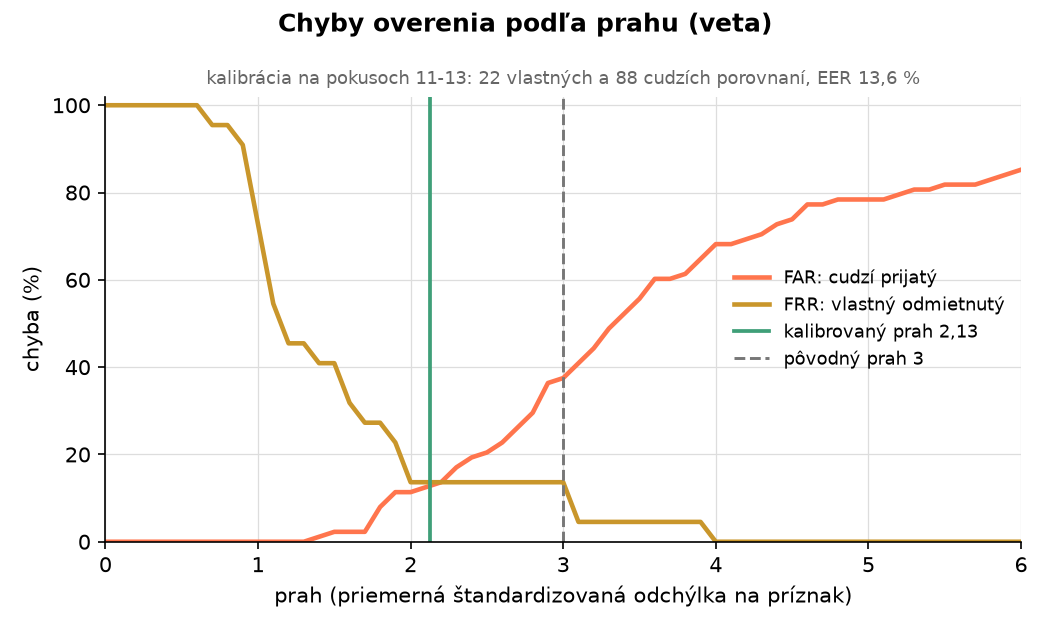
\includegraphics[width=\textwidth]{far_frr_phrase.png}
  \caption{Krivky FAR a FRR podľa prahu}
  \label{fig:farfrr}
\end{figure}

% Obrázok (graf z backend/far_frr.py): rozdelenie skóre.
\begin{figure}[H]
  \centering
  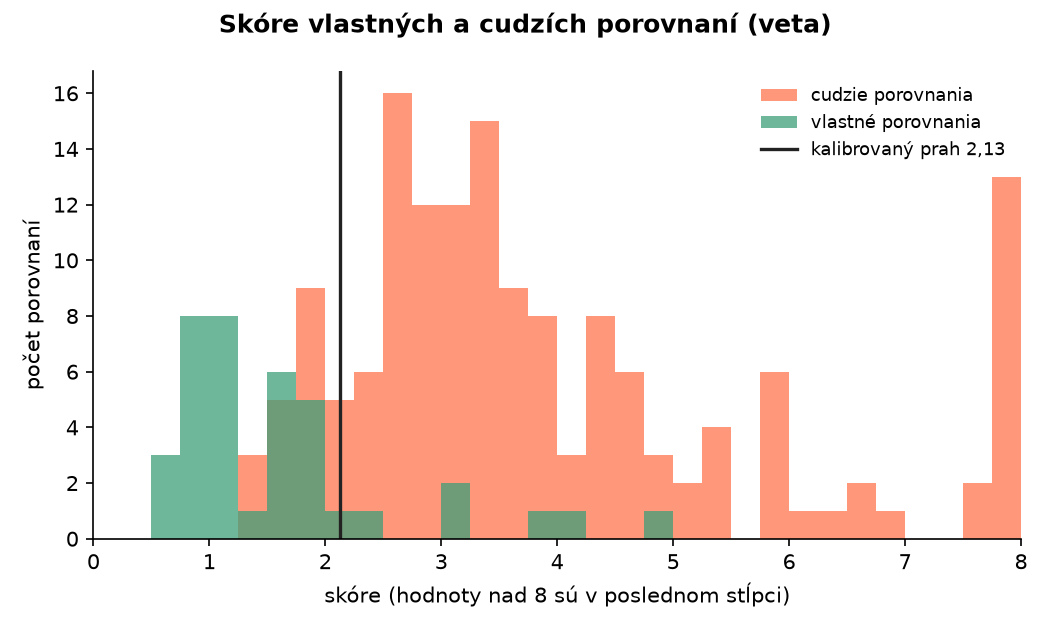
\includegraphics[width=\textwidth]{score_distribution_phrase.png}
  \caption{Rozdelenie skóre vlastných a cudzích porovnaní}
  \label{fig:skore}
\end{figure}

Starý prah 3 je pre overenie príliš voľný: prepustil by viac ako tretinu
cudzích pokusov (35,9\,\%). Nový prah 2,13 túto chybu zníži na 10,9\,\% (7 zo 64
cudzích porovnaní), ale systém potom častejšie odmietne aj vlastný pokus
(18,8\,\% namiesto 12,5\,\%, teda 3 zo 16 pokusov). Čo je lepšie, závisí od
použitia: tam, kde treba chrániť prístup, je dôležitejší nízky FAR. Priemer oboch
chýb na pokusoch 14--15 vyšiel 14,9\,\%, podobne ako EER 13,6\,\% z kalibrácie,
takže prah nie je vyladený len na dáta, z ktorých vznikol.

Obr.~\ref{fig:skore} ukazuje, prečo sa chyby nedajú odstrániť úplne. Skóre
vlastných porovnaní sa drží okolo 1 až 2, skóre cudzích je väčšinou nad 2,5
a má dlhý chvost, ale obe rozdelenia sa trochu prekrývajú.

V režime slova (3 účastníci, 25 testovacích pokusov) vyšiel prah 1,93 a EER
1,7\,\%. Na pokusoch 14--15 bolo FAR 0\,\% a FRR 10\,\%, kým prah 3 by dal FAR
30\,\% a FRR 0\,\%. Dát je tu však málo (10 vlastných a 20 cudzích porovnaní)
a veľká časť patrí jednému človeku (15 z 25 pokusov má Účastník~1), takže to
berieme len ako ilustráciu.

Aj čísla pre vetu sú orientačné. Testovacích vlastných porovnaní je len 16, takže
jeden pokus posunie FRR o 6,25 percentuálneho bodu. Rozdelenie na kalibračné
a testovacie pokusy je pevné (podľa poradia pokusu) a bez krížovej validácie.
Čísla aj grafy sa dajú znovu vytvoriť príkazom \code{python far\_frr.py} (alebo
\code{python far\_frr.py {-}{-}mode word}) v priečinku \code{backend}; skript
vypíše výsledky a nakreslí grafy do \code{docs/figures}.

% ----- Porovnanie vety a slova -----
\subsection{Porovnanie vety a slova}
\label{sec:test-porovnanie}

Na porovnanie režimov slúži koncový bod \code{/api/compare}. Pre každý režim sa podľa protokolu z
podkapitoly~\ref{sec:protokol} zobrazí presnosť top-1 a top-3, podiel pokusov
označených ako neznáme, priemerný čas pokusu a počet príznakov (73 pre vetu,
19 pre slovo). Výpočet sa robí len na účastníkoch, ktorí absolvovali oba
režimy (podkapitola~\ref{sec:porovnanie}); ak ich je menej než dvaja,
server vráti všetky dáta s poznámkou, že porovnanie nie je spravodlivé.

Funkčnosť výpočtu sa overila na syntetických dátach troch účastníkov v oboch
režimoch (správne počty príznakov 73 a 19 a rozdielne priemerné časy pokusu)
a na existujúcich dátach (výsledky pre vetu sa po zavedení režimov nezmenili).
Podľa stavu databázy k 20.~11.~2026 má už aj režim slova dáta od troch
účastníkov (Účastník~1, 3 a 5), ktorí písali aj vetu, takže porovnanie
počítame na týchto troch ľuďoch. Výsledky sú v Tab.~\ref{tab:porovnanie} a na Obr.~\ref{fig:porovnanie}.

% Tabuľka: Porovnanie vety a slova na troch spoločných účastníkoch.
\begin{table}[!htbp]
  \centering
  \small
  \caption{Porovnanie vety a slova}
  \label{tab:porovnanie}
  \begin{tabularx}{\textwidth}{|Y|C|C|}
    \hline
    \rowcolor[gray]{0.9} \textbf{Ukazovateľ} & \textbf{Veta} & \textbf{Slovo} \\
    \hline
    Počet príznakov & 73 & 19 \\
    \hline
    Testovacie pokusy (11--15) & 28 & 25 \\
    \hline
    Top-1 & 85,71\,\% & 100,0\,\% \\
    \hline
    Top-3 & 100,0\,\% & 100,0\,\% \\
    \hline
    Podiel pokusov označených ako neznáme & 3,57\,\% & 0,0\,\% \\
    \hline
    Priemerný čas pokusu & 9,6~s & 2,7~s \\
    \hline
  \end{tabularx}
\end{table}

% Obrázok (graf generuje server po každom uložení relácie): presnosť vety a slova.
\begin{figure}[H]
  \centering
  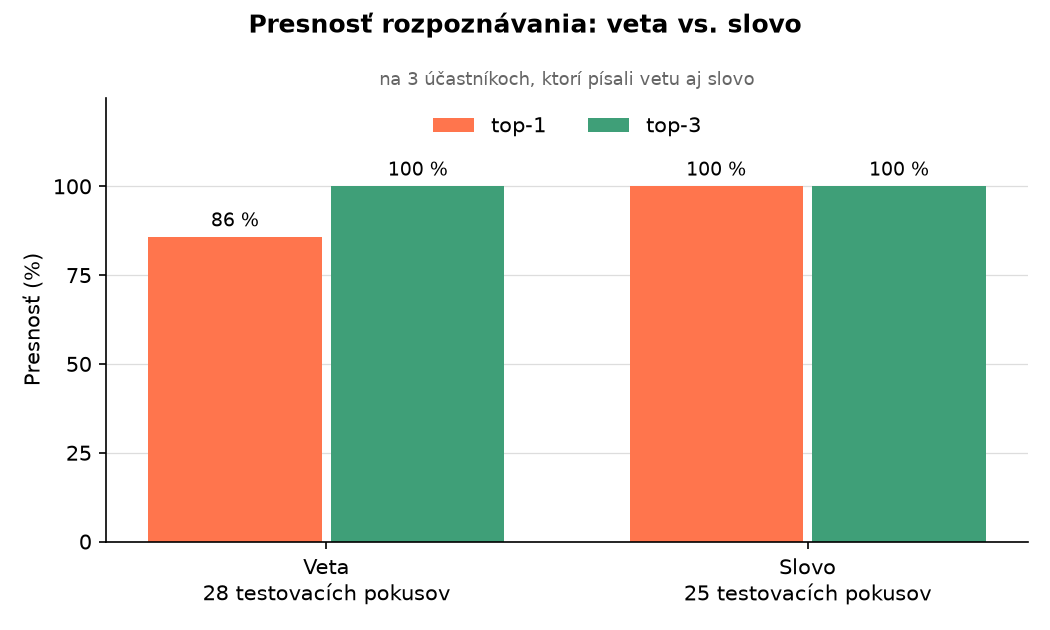
\includegraphics[width=\textwidth]{accuracy_chart.png}
  \caption{Presnosť vety a slova}
  \label{fig:porovnanie}
\end{figure}

Čísla netreba preceňovať. Pri troch šablónach je náhodný odhad pre top-1 33\,\%
a top-3 je vždy 100\,\%, lebo v zozname sú všetci traja účastníci. Pokusy sú
rozdelené nerovnomerne: pri vete je 20 z 28 pokusov od Účastníka~5, pri slove
15 z 25 od Účastníka~1. Šablóna Účastníka~1 pre slovo vznikla zo všetkých troch
jeho relácií, pre vetu má len jednu, takže náskok slova môže byť čiastočne len
dôsledok väčšieho množstva dát. Spoľahlivo vieme povedať iba toľko, že pokus so
slovom trvá asi 3,5-krát kratšie (2,7~s oproti 9,6~s) a že na týchto troch
ľuďoch slovo nedopadlo horšie ako veta.
